\documentclass[aspectratio=169]{beamer}
\usetheme{metropolis}
\usepackage{graphicx}
\usepackage{booktabs}
\usepackage{siunitx}
\usepackage{amsmath}
\usepackage{hyperref}

\graphicspath{{../report/figures/}}

\title{FEA of Sustainable Helmet Materials}
\subtitle{under EN 397 Impact}
\author{Your Name}
\institute{ECM3175 Final Year BEng Mechanical Engineering\\University of Exeter}
\date{April 2026}

\begin{document}

\begin{frame}
  \titlepage
\end{frame}

\begin{frame}{The Problem Context}
  \begin{itemize}
    \item \textbf{Environmental Impact:} Standard PPE (e.g., Virgin HDPE) has a high environmental cost.
    \item \textbf{The Challenge:} Transitioning to sustainable alternatives without compromising safety.
    \item \textbf{Regulatory Standard:} EN 397 is the safety-critical regulation for industrial helmets.
  \end{itemize}
\end{frame}

\begin{frame}{Material Candidates}
  \begin{table}
    \centering
    \begin{tabular}{lcc}
      \toprule
      \textbf{Material} & \textbf{Modulus (GPa)} & \textbf{Yield Stress (\si{kg/mm^2})} \\
      \midrule
      Virgin HDPE (Baseline) & 1.00 & 2.55 \\
      ABS Plastic & 2.10 & 4.08 \\
      Bamboo-HDPE (30\% wt) & 1.50 & 3.26 \\
      Recycled PC (rPC) & 2.30 & 6.12 \\
      \bottomrule
    \end{tabular}
  \end{table}
\end{frame}

\begin{frame}{Methodology \& Impact Setup}
  \begin{columns}
    \begin{column}{0.5\textwidth}
      \begin{itemize}
        \item \textbf{Setup:} Galilean upward velocity shift applied to helmet/headform.
        \item \textbf{Velocity:} \SI{4.43}{m/s} against a rigid ceiling.
        \item \textbf{Solver:} LS-DYNA Explicit Dynamics.
      \end{itemize}
    \end{column}
    \begin{column}{0.5\textwidth}
      \centering
      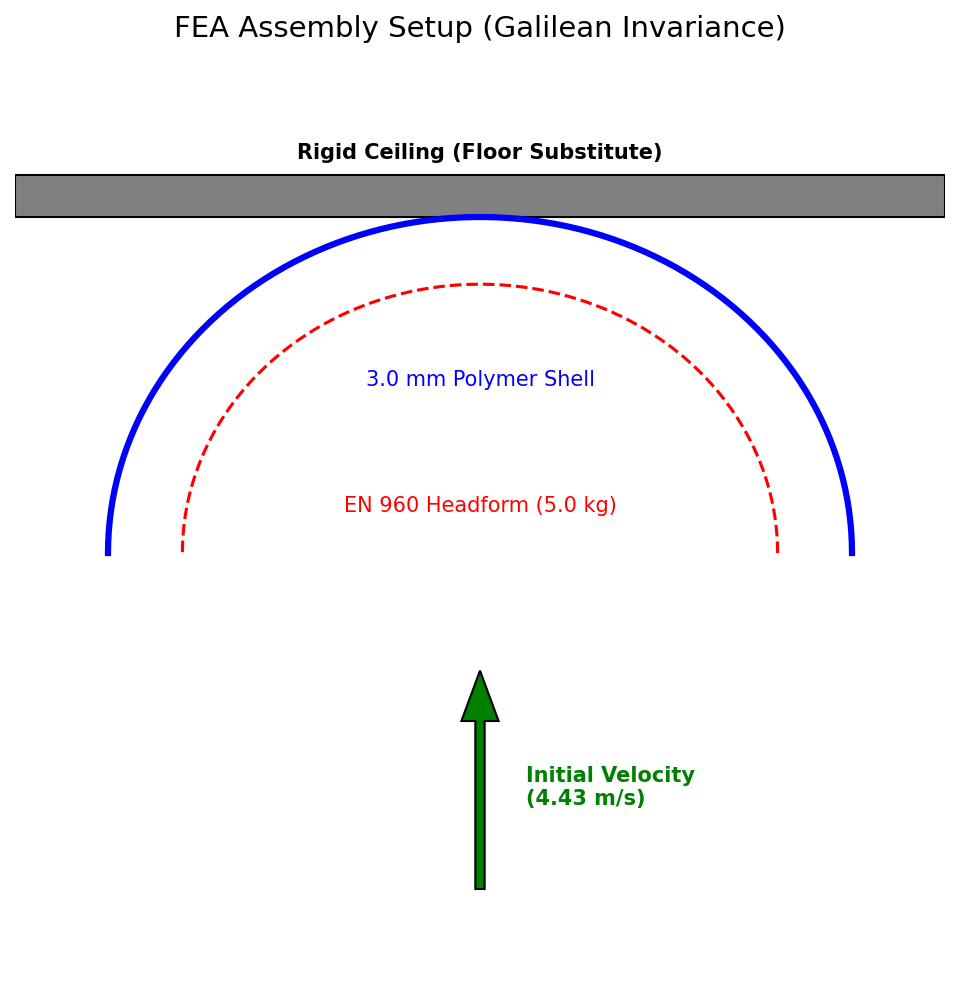
\includegraphics[width=\textwidth]{Assembly_Setup.png}
    \end{column}
  \end{columns}
\end{frame}

\begin{frame}{Computational Rigor \& Stability}
  \begin{columns}
    \begin{column}{0.5\textwidth}
      \begin{itemize}
        \item \textbf{Time Integration:} Explicit Central Difference Method.
        \item \textbf{Stability:} CFL condition ($\Delta t \leq L_{min}/c$).
        \item \textbf{Validation:} \SI{0.00}{J} hourglass energy, $< 0.04\%$ energy drift.
        \item \textbf{Mesh:} Convergence achieved at \SI{2}{mm} (~42,000 elements).
      \end{itemize}
    \end{column}
    \begin{column}{0.5\textwidth}
      \centering
      
\includegraphics[width=\textwidth]{Helmet_Mesh.png}
    \end{column}
  \end{columns}
\end{frame}

\begin{frame}{Phase 2: EN 397 Force Transmission}
  \begin{columns}
    \begin{column}{0.5\textwidth}
      \begin{itemize}
        \item \textbf{Criterion:} Transmitted force must be $< \SI{5.0}{kN}$.
        \item \textbf{Results:} All materials pass.
        \begin{itemize}
          \item Virgin HDPE: \SI{4.05}{kN}
          \item ABS: \SI{2.25}{kN}
          \item Bamboo-HDPE: \SI{4.51}{kN}
          \item Recycled PC: \SI{4.54}{kN}
        \end{itemize}
        \item \textbf{Signal Processing:} Data filtered using SAE J211 CFC 60 to isolate macroscopic deceleration.
      \end{itemize}
    \end{column}
    \begin{column}{0.5\textwidth}
      \centering
      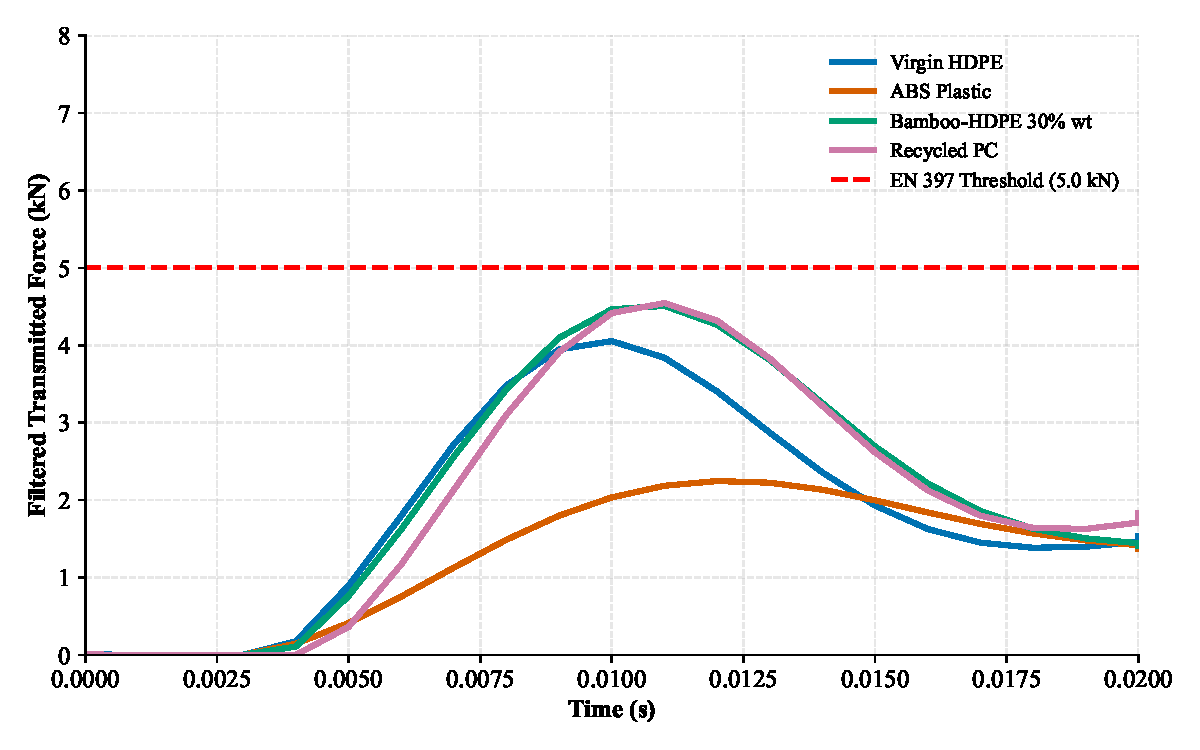
\includegraphics[width=\textwidth]{Phase2_ForceTransmission_Filtered.pdf}
    \end{column}
  \end{columns}
\end{frame}

\begin{frame}{Phases 3 \& 4: Energy Absorption Mechanisms}
  \begin{itemize}
    \item \textbf{High Ductility (Virgin HDPE):}
      \begin{itemize}
        \item Absorbs impact energy primarily through internal strain yielding and plastic deformation.
        \item Energy Absorption Ratio: 55.3\%.
        \item Crush Depth: \SI{18.42}{mm}.
      \end{itemize}
    \item \textbf{High Modulus (ABS, rPC):}
      \begin{itemize}
        \item Relies on load distribution due to increased flexural stiffness, distributing forces across a wider EPS liner area.
        \item rPC Energy Absorption Ratio: 33.5\%, Crush Depth: \SI{10.23}{mm}.
      \end{itemize}
  \end{itemize}
\end{frame}

\begin{frame}{Phase 5: 30$^\circ$ Oblique Impact}
  \begin{columns}
    \begin{column}{0.5\textwidth}
      \begin{itemize}
        \item \textbf{Objective:} Advanced simulation beyond standard EN 397 to evaluate real-world complex impacts.
        \item \textbf{Setup:} 30$^\circ$ angled impact surface.
        \item \textbf{Focus:} Rotational kinematics and tangential frictional interactions.
      \end{itemize}
    \end{column}
    \begin{column}{0.5\textwidth}
      \centering
      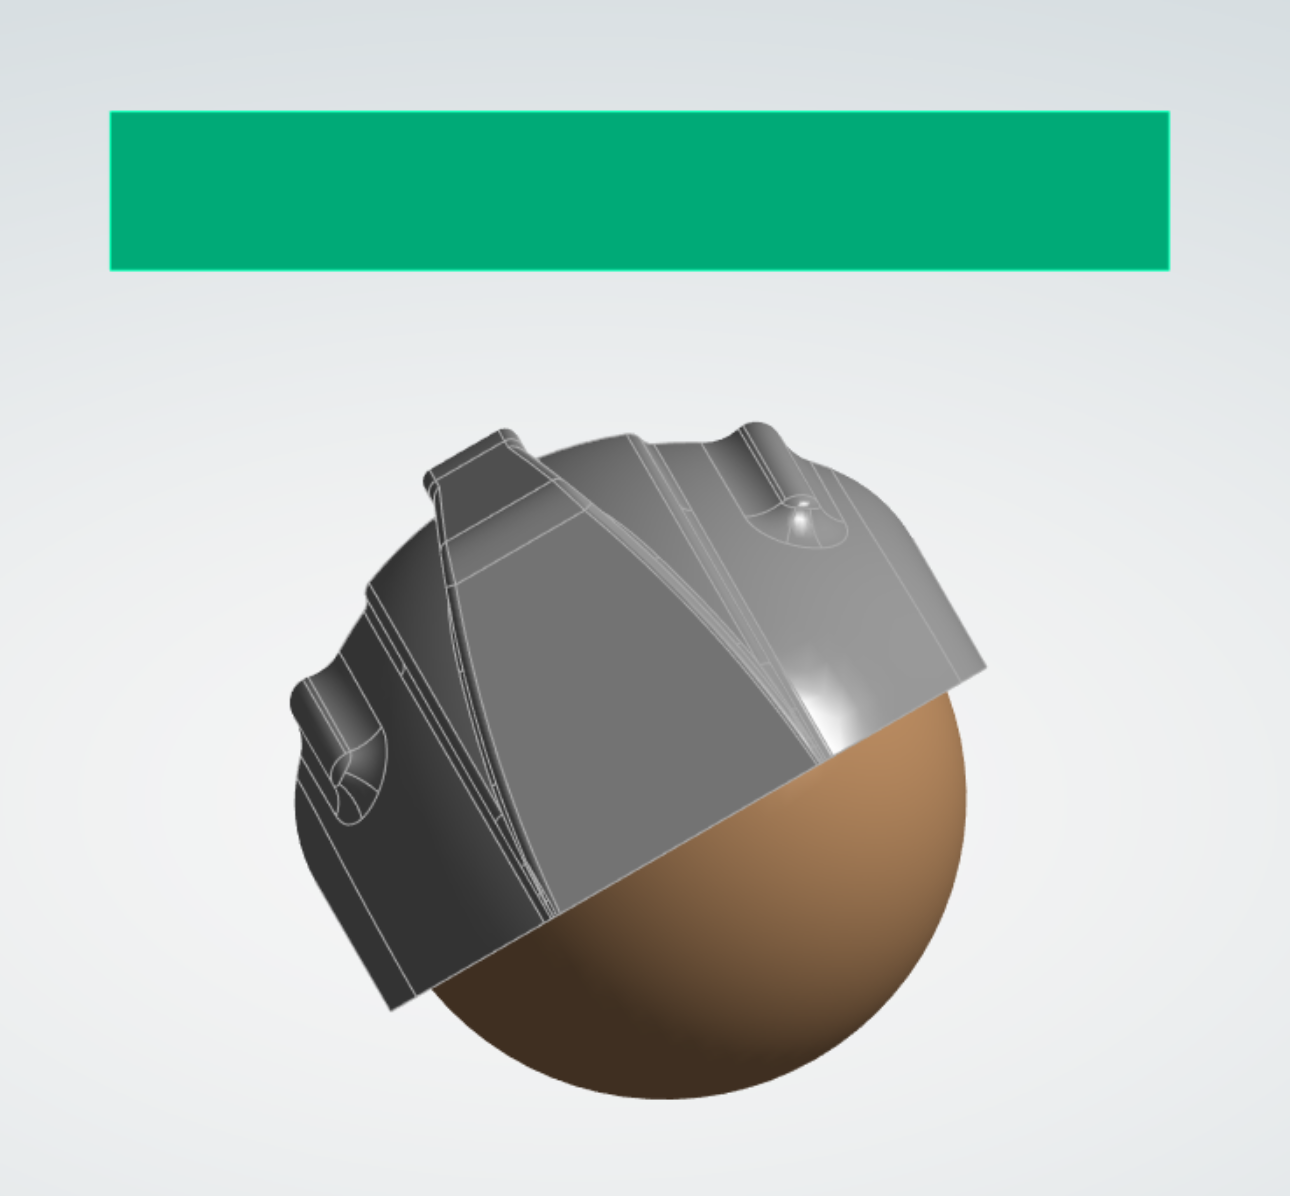
\includegraphics[width=\textwidth]{oblique_setup_view.png}
    \end{column}
  \end{columns}
\end{frame}

\begin{frame}{Rotational Kinematics (Key Finding)}
  \begin{columns}
    \begin{column}{0.5\textwidth}
      \begin{itemize}
        \item \textbf{rPC Performance:} Achieved a 74\% reduction in peak rotational acceleration compared to Virgin HDPE (\SI{896}{rad/s^2} vs \SI{3482}{rad/s^2}).
        \item \textbf{Mechanism:} Reduced tangential frictional interaction. Higher flexural modulus limits localized surface deformation, unlike the plastic deformation seen in HDPE.
      \end{itemize}
    \end{column}
    \begin{column}{0.5\textwidth}
      \centering
      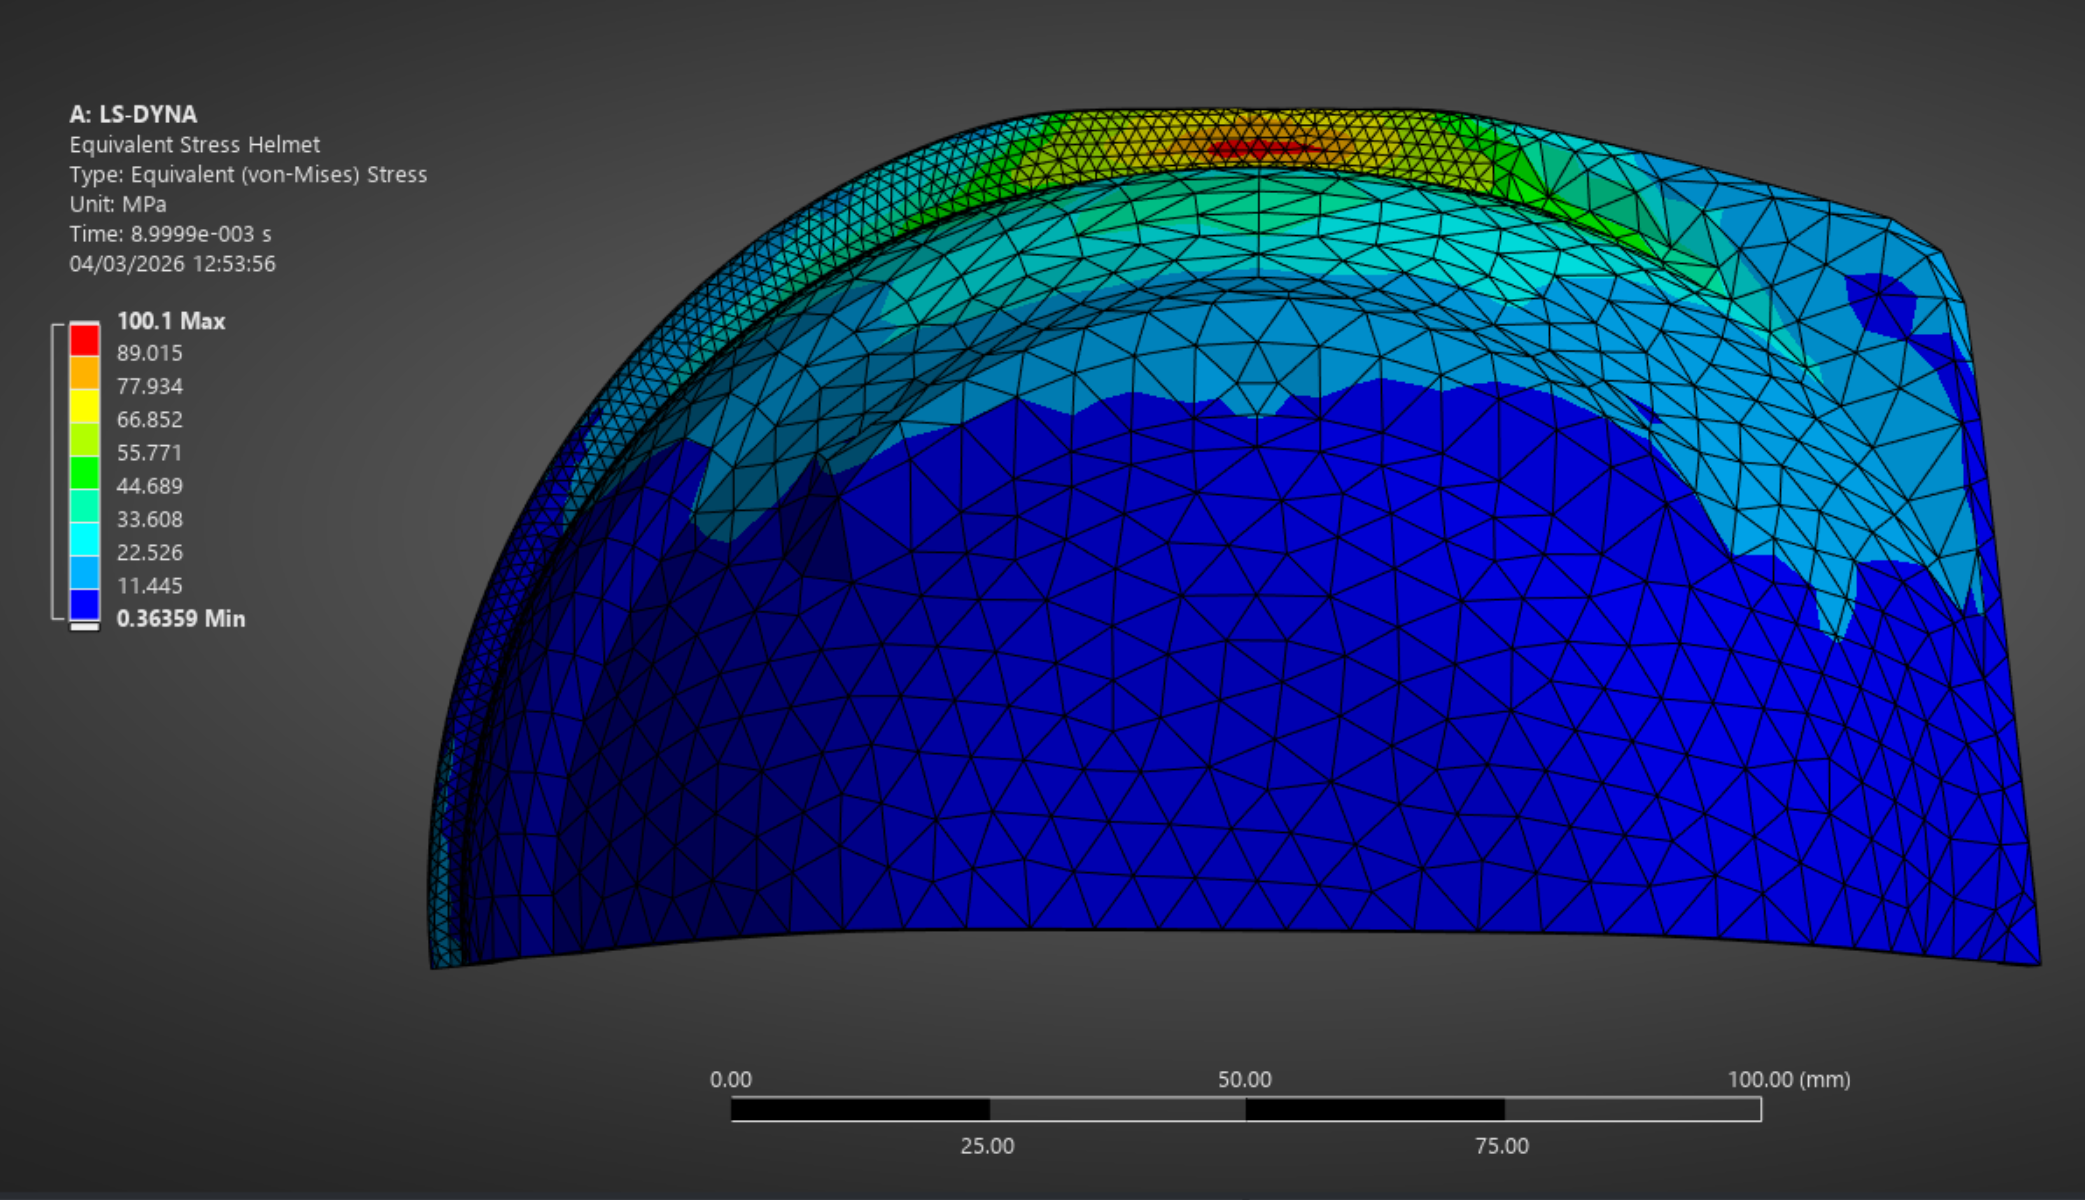
\includegraphics[width=0.8\textwidth]{stress_oblique_section_rpc.png}\\
      \vspace{0.2cm}
      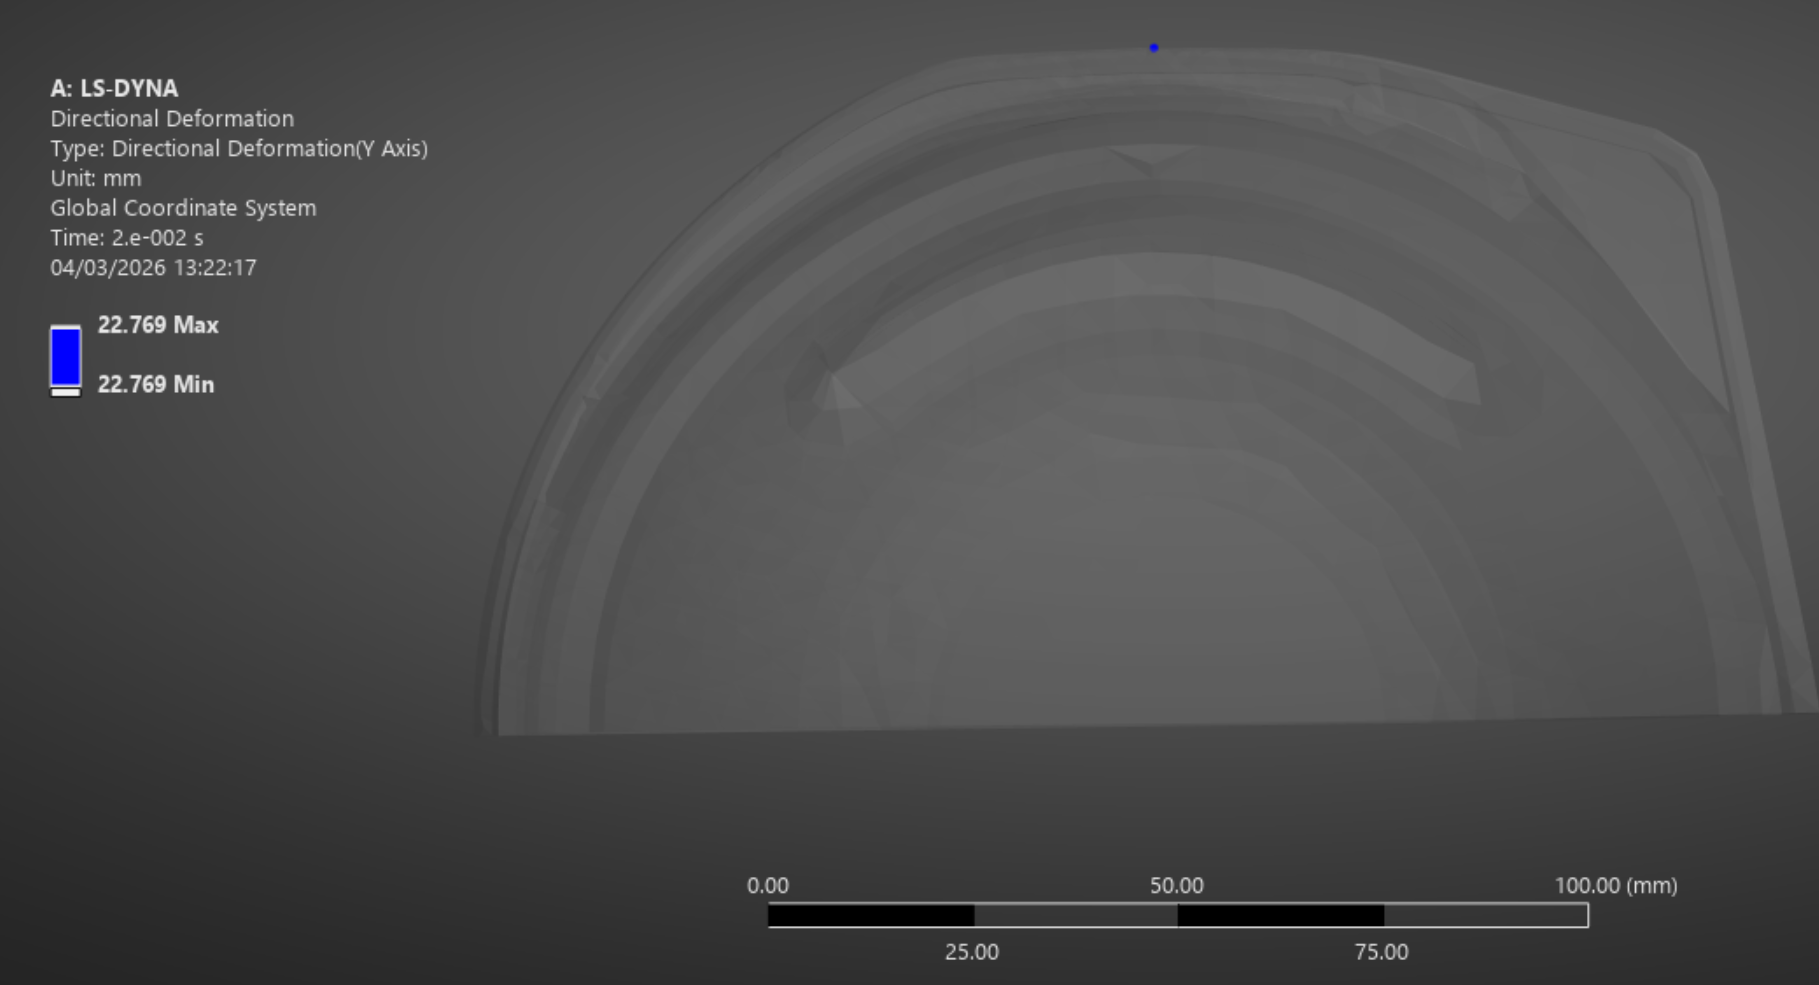
\includegraphics[width=0.8\textwidth]{stress_oblique_section_hdpe.png}
    \end{column}
  \end{columns}
\end{frame}

\begin{frame}{Project Management \& Risk}
  \begin{columns}
    \begin{column}{0.5\textwidth}
      \begin{itemize}
        \item \textbf{Execution:} Systematic adherence to the project Gantt chart.
        \item \textbf{Safety:} Implementation of a comprehensive Systematic Risk Register.
        \item \textbf{Audit:} Units synchronized across all models (\si{GPa}/\si{kg/mm^2}).
      \end{itemize}
    \end{column}
    \begin{column}{0.5\textwidth}
      \centering
      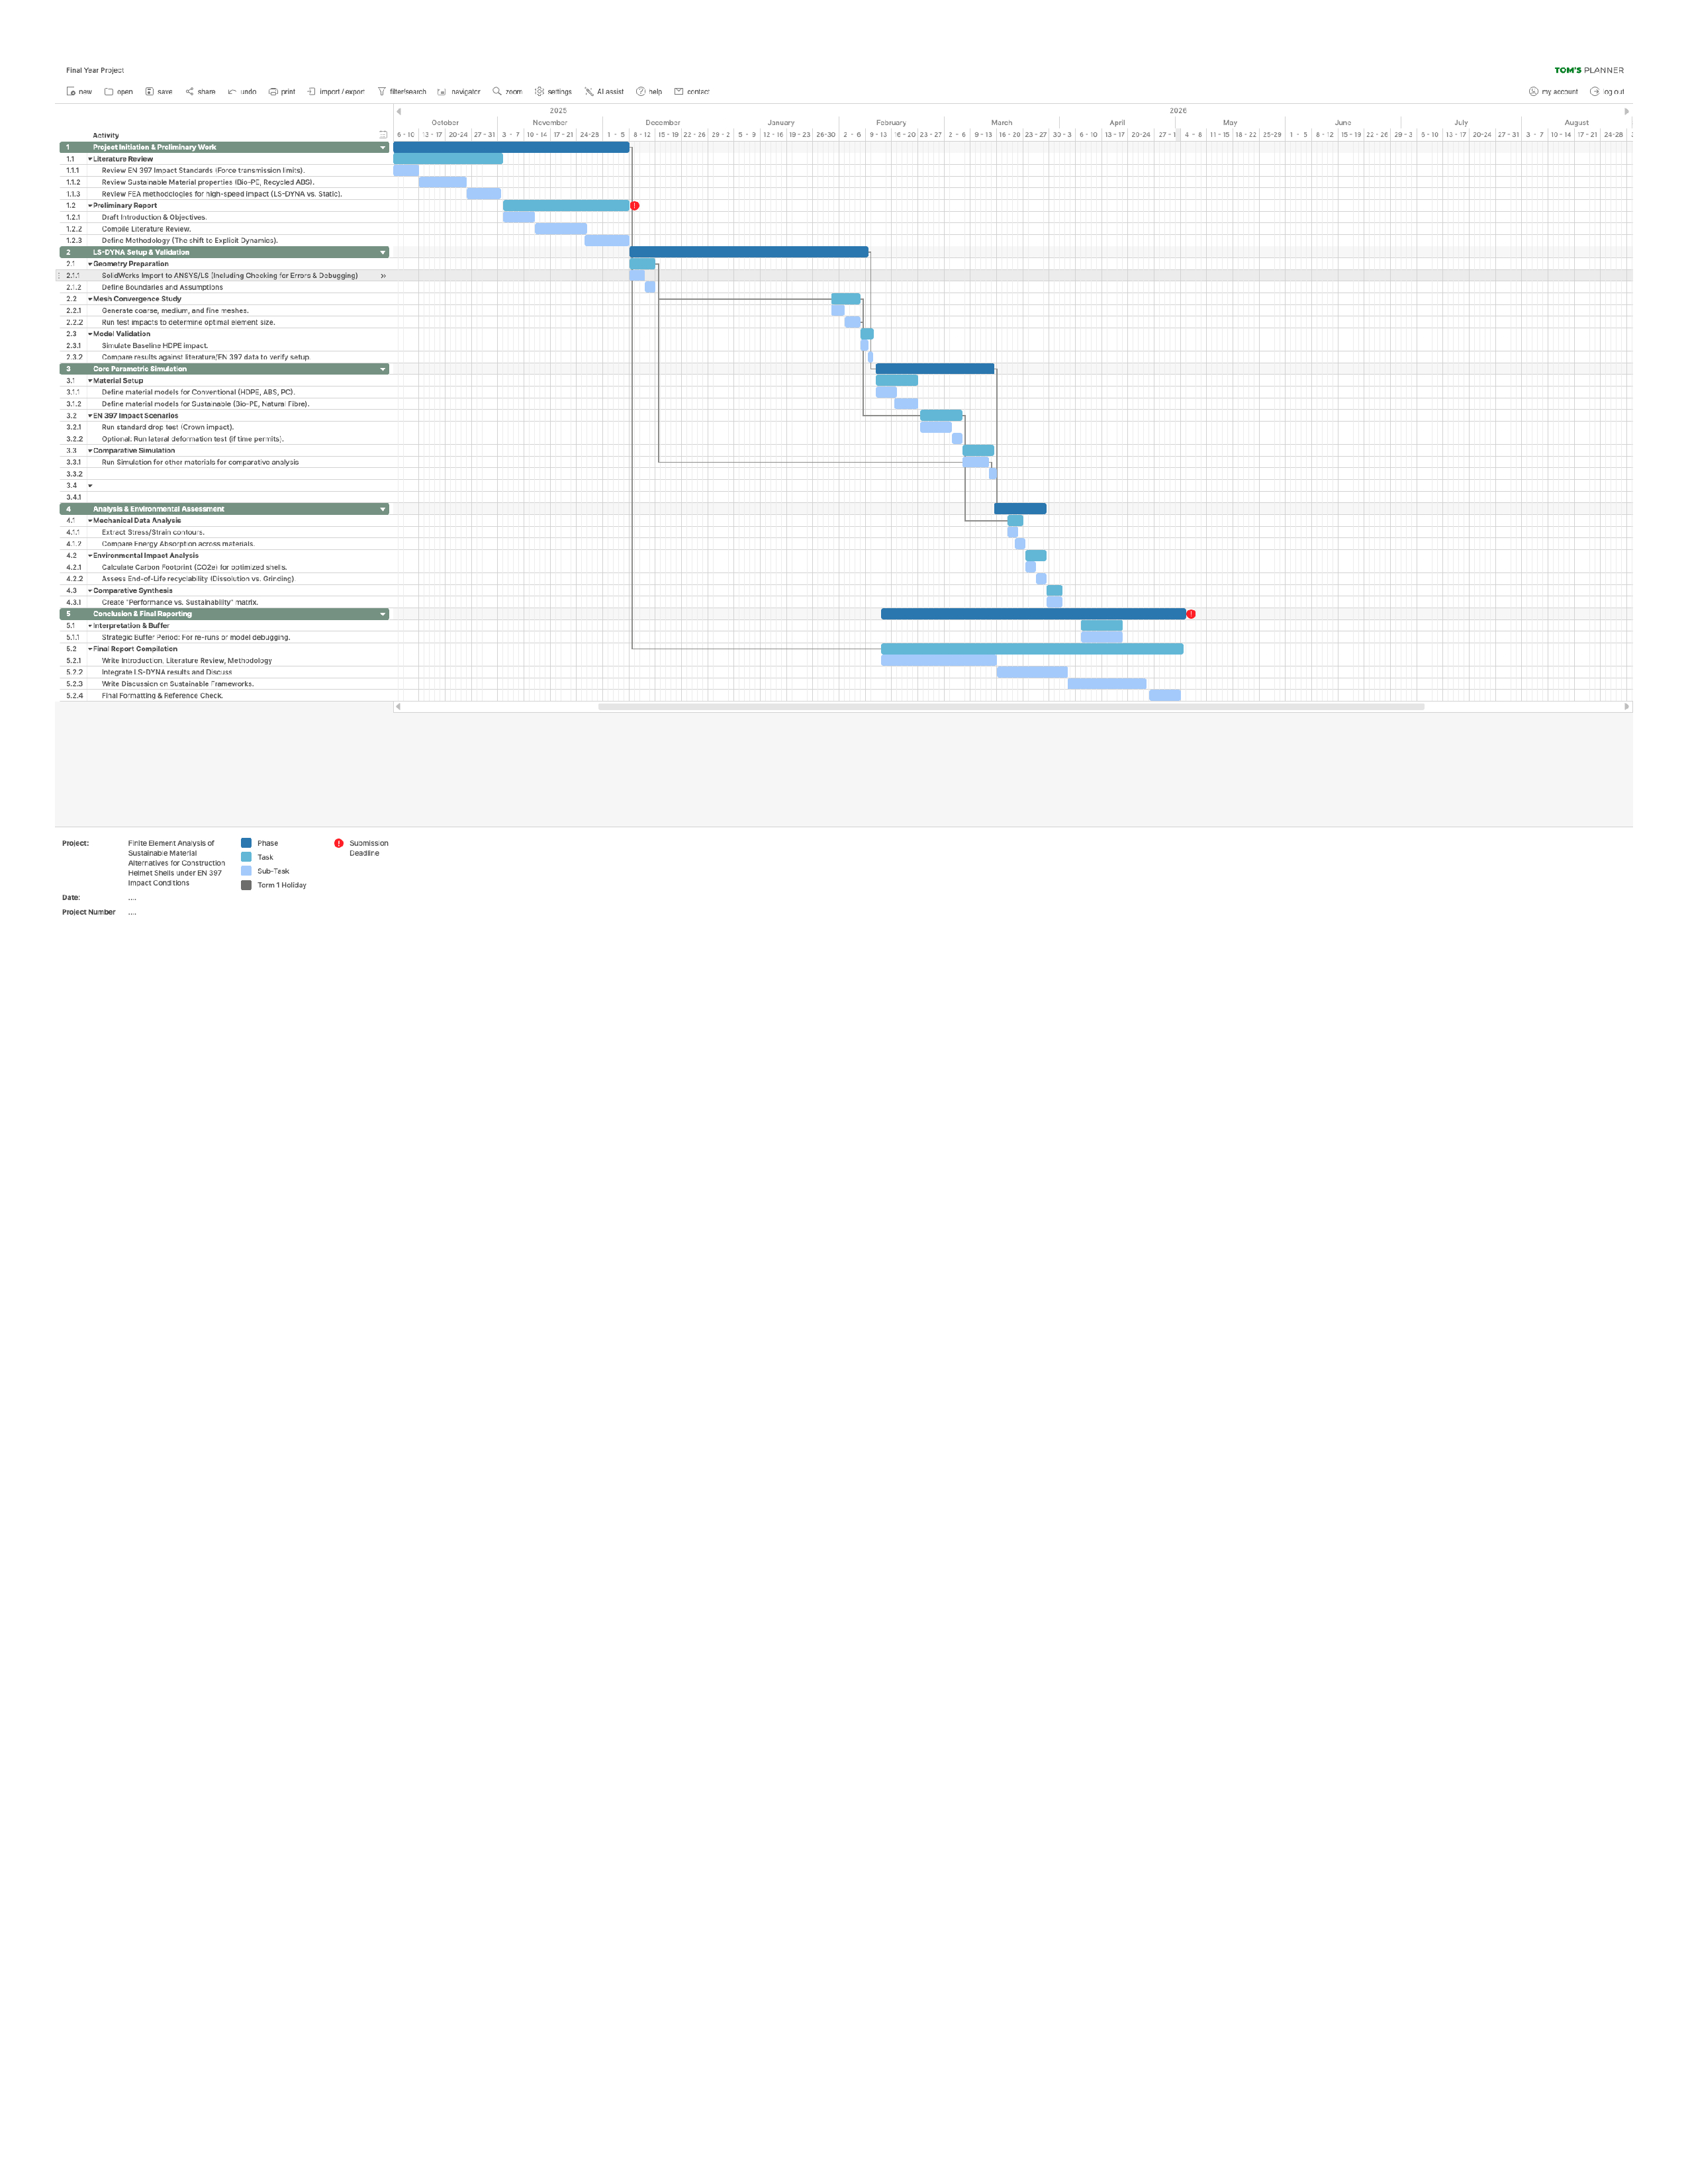
\includegraphics[width=\textwidth]{gantt_image.png}
    \end{column}
  \end{columns}
\end{frame}

\begin{frame}{Conclusion}
  \begin{itemize}
    \item \textbf{Validation:} Sustainable alternatives (rPC, Bamboo-HDPE) provide sufficient structural protection and meet strict EN 397 regulations.
    \item \textbf{Superiority in Complex Impacts:} rPC outperforms traditional materials in oblique impacts by mitigating rotational acceleration.
    \item \textbf{Impact:} Significant reduction in the environmental footprint of PPE without compromising safety-critical performance.
  \end{itemize}
\end{frame}

\begin{frame}
  \centering
  \Huge \textbf{Questions?}
\end{frame}

\end{document}
